\documentclass[12]{article}

\usepackage{gensymb}
\usepackage{listings}
\usepackage{float}
\usepackage{float}
\usepackage{booktabs}
\usepackage{multirow}

\usepackage{amsmath}
\usepackage{booktabs,tabularx}
\usepackage{gensymb}

\usepackage{float}
\usepackage{booktabs}
\usepackage{multirow}
\usepackage{graphicx}
\usepackage{subcaption}
\usepackage{mwe}
\usepackage{amsmath}
\usepackage{ushort}
\usepackage[utf8]{inputenc}
\usepackage[T1]{fontenc}
\setlength{\oddsidemargin}{0.25 in}
\setlength{\evensidemargin}{-0.25 in}
\setlength{\topmargin}{-0.6 in}
\setlength{\textwidth}{6.5 in}
\setlength{\textheight}{8.5 in}
\setlength{\headsep}{0.75 in}
\setlength{\parindent}{0 in}
\setlength{\parskip}{0.1 in}
\usepackage{geometry}
\usepackage{textcomp}
\usepackage[table,xcdraw]{xcolor}
\usepackage{hyperref}
\usepackage{cancel}

\hypersetup{
    colorlinks,
    citecolor=black,
    filecolor=black,
    linkcolor=blue,
    urlcolor=blue
}

\usepackage{graphicx}
\usepackage[inkscapeformat=pdf,inkscapelatex=false]{svg}
\graphicspath{ {./figs/} }

\begin{document}

\begin{titlepage}
\newcommand{\HRule}{\rule{\linewidth}{0.5mm}}
\setlength{\topmargin}{0 in}
\begin{center}
\begin{figure}[!h]
\centering

\includegraphics [width=0.3\textwidth]{eelogo.png}
\end{figure}

\vspace{10mm}
\Huge{MIDDLE EAST TECHNICAL UNIVERSITY}\\
\vspace{5mm}
{\LARGE ELECTRICAL \& ELECTRONICS ENGINEERING}\\

\HRule\\[0.4cm]
\textsc{\Large{EE462 - UTILIZATION OF ELECTRICAL ENERGY}}\\
\textsc{\Large{Homework V}}
\HRule\\[0.4cm]

\vspace{3mm}

\end{center}
\begin{minipage}{0.5\textwidth}
		\begin{flushleft}
			\large
			Emre Deniz  \textsc{Şenel - 2167237}\\
		\end{flushleft}
	\end{minipage}


\vspace{10mm}
\begin{center}
\large{18.05.2020}
\end{center}

\end{titlepage}
\tableofcontents
\newpage
\section{Part A - Pre Design Stage}
\subsection{Q1}
In this part, we are asked to calculate the rated torque of the motor.

\begin{equation}
    T_{rated} = \dfrac{P_{nominal}}{\omega_{nominal}} = \dfrac{400kW}{50\pi} = 2546 \; Nm
\end{equation}

\subsection{Q2}
In this part, we are going to calculate the rated frequency of the machine, and depending on the maximum frequency, we will choose a switching frequency.

\begin{equation}
    f_{m,max} = \dfrac{2250}{60} = 37.5 Hz,
\end{equation}

\begin{equation}
    f_{max} = f_{m,max} pp = 75 Hz
\end{equation}

As we increase the switching frequency, the losses will increase. So, we need to choose an adequate switching frequency. Also, to eliminate the lower harmonics we are going to choose a large switching frequency.

We choose the switching frequency as

\begin{equation}
    f_s = 3000
\end{equation}

\subsection{Q3}
% DC link design, its simulation results
\section{Part B: Sinusoidal PWM}
\subsection{Q1}
%simulation from 90% speed to 100% speed. Plot speed vs time, 3 phase line to line voltages, 3 phase line currents, torque vs time, d-q currents, transition time

\subsection{Q2}
% when rated speed, make TL = 0, what happens, show graphs

\subsection{Q3}
%when no load, reverse the reference, if feasible? design a braking resistor, plot speed vs time,  3 phase line currents, d-q currents, dc link voltage,  

\subsection{Q4}

\section{Part C - Space Vector PWM}
\subsection{Q1}
\subsubsection{Q1-1}

In the Fig \ref{fig:s2} below, we can observe the speed vs time graph of the pmsm motor. Here, we can see that the motor is speeding up from its 90\% rated speed to its rated speed. 

\begin{center}
\begin{figure}[H]
\centering
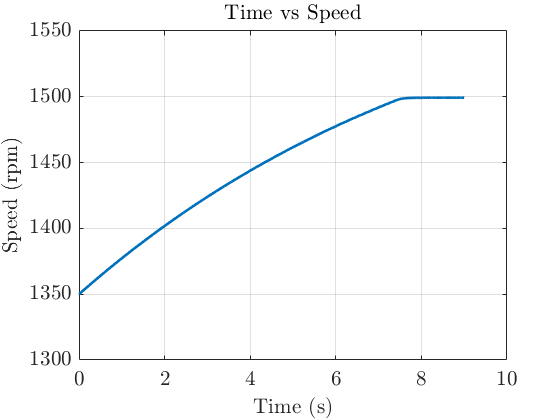
\includegraphics [width = 10 cm]{figs/speed.png}
\caption{Speed vs time graph of the motor}
\label{fig:s2}
\end{figure}
\end{center}

In the Fig. \ref{fig:3line} and Fig. \ref{fig:3line_1} below, we can observe the line to line voltage vs time

\begin{figure}[H]
        \centering
        \begin{subfigure}[b]{0.475\textwidth}
            \centering
            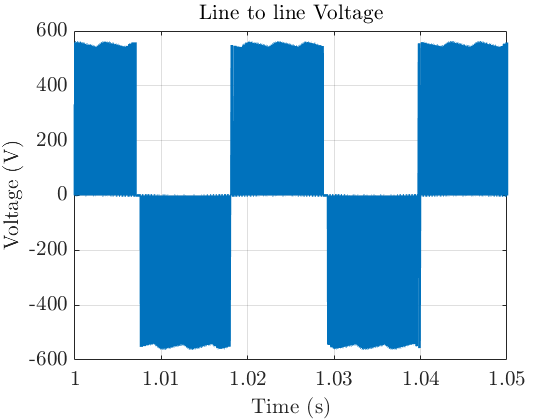
\includegraphics[width = 7 cm]{figs/lineVoltage.png}
            \caption{Line to line voltage}
            \label{fig:3line}
        \end{subfigure}
        \hfill
        \begin{subfigure}[b]{0.475\textwidth}  
            \centering 
            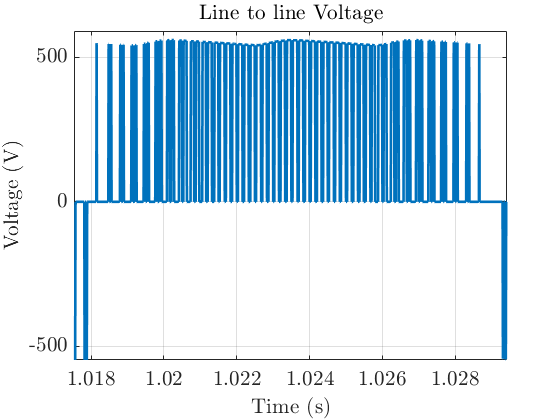
\includegraphics[width = 7 cm]{figs/lineVoltage_zoom.png}
            \caption{Line to line voltage, one cycle}
            \label{fig:3line_1}
        \end{subfigure}
        \caption{Line to line voltage general (a) and one cycle (b)}
        \label{fig:3phase}
        \end{figure}
        
In the Fig. \ref{fig:lineC} and Fig. \ref{fig:lineC_1} below, we can observe the phase current, Fig. \ref{fig:lineC} is the current while the motor is speeding up, and Fig. \ref{fig:lineC_1} shows the current when motor reaches its steady state speed.

\begin{figure}[H]
        \centering
        \begin{subfigure}[b]{0.475\textwidth}
            \centering
            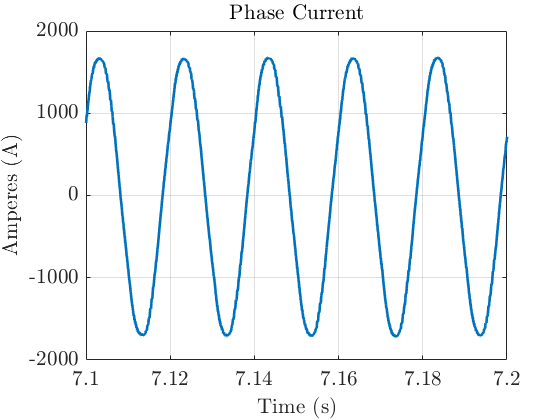
\includegraphics[width = 7 cm]{figs/phase_steady.png}
            \caption{Line to line voltage}
            \label{fig:lineC}
        \end{subfigure}
        \hfill
        \begin{subfigure}[b]{0.475\textwidth}  
            \centering 
            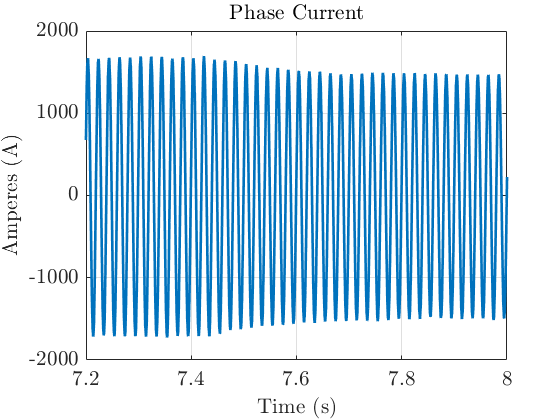
\includegraphics[width = 7 cm]{figs/phase_transient.png}
            \caption{Line to line voltage, one cycle}
            \label{fig:lineC_1}
        \end{subfigure}
        \caption{Phase current speeding up (a) and transient to the steady state (b)}
        \label{fig:3phase}
        \end{figure}
        
In the Fig. \ref{fig:t2} below, we can observe the machine torque vs time graph. It shows that the torque is increasing due to the load characteristic. Also, d-q currents in the stator shows a similar transient. Since torque and $i_q$ currents are directly proportional to each other, it is easy to see relation between them.

\begin{figure}[H]
        \centering
        \begin{subfigure}[b]{0.475\textwidth}
            \centering
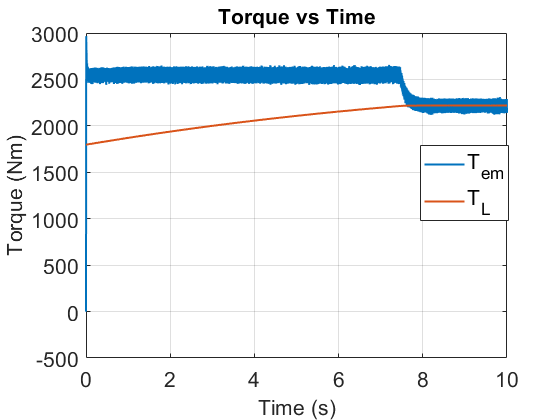
\includegraphics [width= 8 cm]{figs/torque_sv_new.png}
\caption{Torque vs time graph of the motor}
\label{fig:t2}
        \end{subfigure}
        \hfill
        \begin{subfigure}[b]{0.475\textwidth}  
            \centering
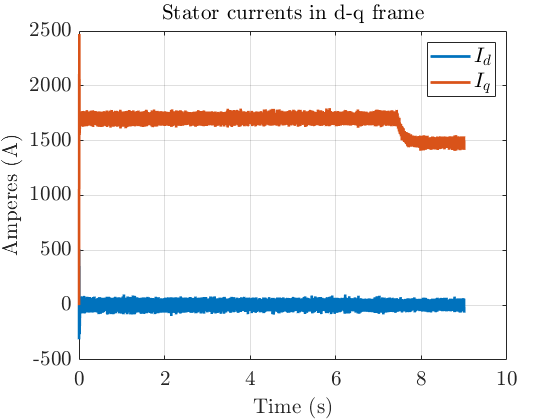
\includegraphics [width= 8 cm]{figs/d_q_currents.png}
\caption{Torque vs time graph of the motor}
\label{fig:dq2}
        \end{subfigure}
        \caption{Phase current speeding up (a) and transient to the steady state (b)}
        \label{fig:3phase}
        \end{figure}



\subsubsection{Q1-2}


In the Fig. \ref{fig:sv_tl0_torque} below, we can observe the machine torque vs time graph. It shows that the torque is decreasing after time step $t=1s$ where we decrease the load torque to zero.

\begin{center}
\begin{figure}[H]
\centering
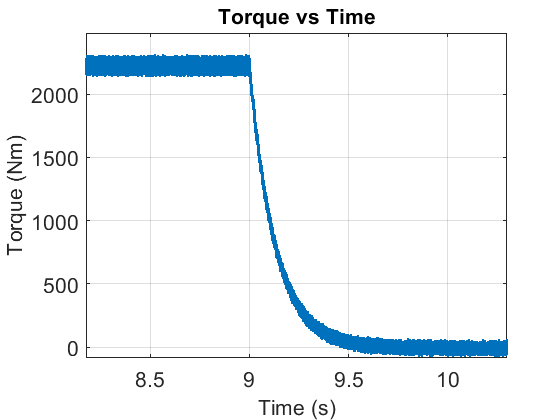
\includegraphics [width= 10 cm]{figs/sv_tl0_torque.png}
\caption{Torque vs time graph of the motor}
\label{fig:sv_tl0_torque}
\end{figure}
\end{center}

In this part, we lower the mechanical torque to the zero as we operating in rated conditions. we expect our phase currents to decrease and of course the $i_q$ current which deploys torque to decrease. 

In the Fig. \ref{fig:sv_3phase_c} below, we can observe the phase currents vs time
        
        \begin{figure}[H]
        \centering
        \begin{subfigure}[b]{0.475\textwidth}
              \centering
        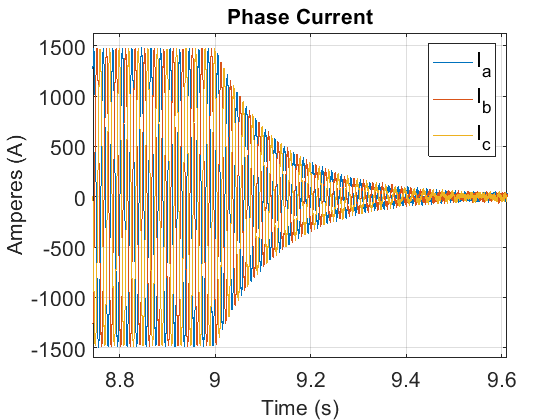
\includegraphics[width = 8 cm]{figs/sv_tl0_abc.png}
        \caption{Motor line currents during transient}
        \label{fig:sv_tl0_p}
        \end{subfigure}
        \hfill
        \begin{subfigure}[b]{0.475\textwidth}  
            \centering
        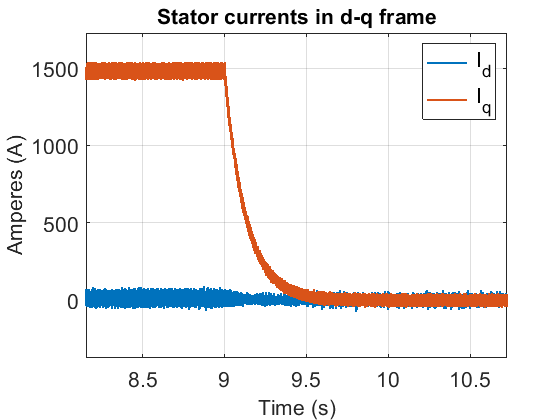
\includegraphics[width = 8 cm]{figs/sv_tl0_dq.png}
        \caption{Motor stator d-q currents during transient}
        \label{fig:sv_tl0_dq}
        \end{subfigure}
        \caption{Line to line voltage general (a) and one cycle (b)}
        \label{fig:sv_3phase_c}
        \end{figure}
        
We can observe that the phase currents are lowering due to decrease in the torque. We know that the torque is directly proportional to the $i_q$ current, and a decrease in the $i_q$ while keeping $i_d$ constant will decrease line currents. After the transient, we have a noise in the line currents due to the inertia of the motor and the noise in the controllers.
        
As we observe, the $I_q$ current was it in rated value to apply rated torque at rated speed, then suddenly we decrease the load torque. Due to the controller, $i_q$ current decreases to $0$ where it provides zero torque, however, there are noise due to the controller circuit and motor itself.

\subsubsection{Q1-3}


We know that during the braking time, the motor supplies current to the utility side, and if we do not have a full quadrant operation or back to back rectifiers, it is not possible to supply energy from load to the grid. In this case of operation as we have in this project, it is not possible to have a current into the grid because of the diode rectifier. So, the solution must be braking resistance. During transient time, the energy stored on the load and the motor can be discharged through this resistor. It prevents the circuit from burn-outs and excessive heating. The braking resistance selection of us is $R = 0.5 \ohm$

In the Fig. \ref{fig:rev} we can observe that after we reverse the reference speed at time $t=1$ the motor speed decreases to 0, and then reversely increases to its final value. Meanwhile, due to the reversal, a negative torque is applied to the motor and it creates a current in the negative direction. This current should be discharged in order to prevent burn outs in the circuitry. Because of this simple phenomenon we introduce a braking resistance to the circuit.

\begin{figure}[H]
        \centering
        \begin{subfigure}[b]{0.475\textwidth}
            \centering
            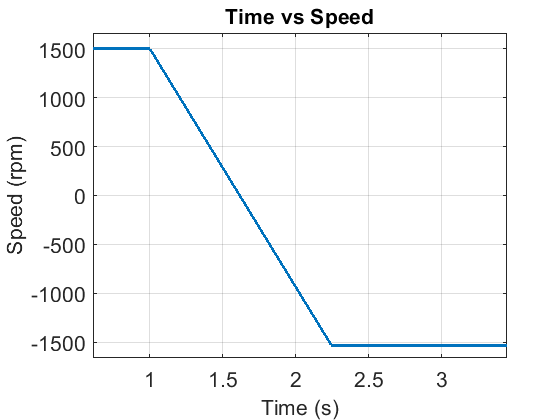
\includegraphics[width = 8 cm]{figs/reverse_sv_speed.png}
            \caption{Speed }
            \label{fig:r_s}
        \end{subfigure}
        \hfill
        \begin{subfigure}[b]{0.475\textwidth}  
            \centering 
            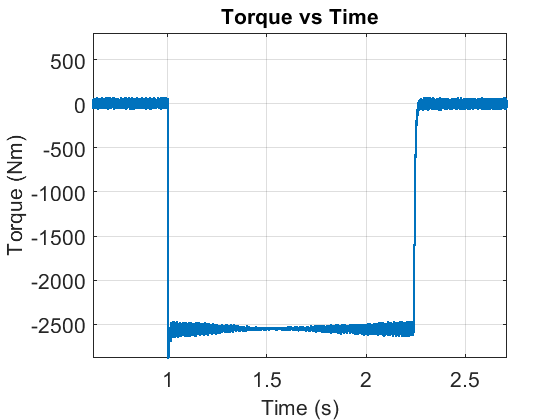
\includegraphics[width = 8 cm]{figs/reverse_sv_torque.png}
            \caption{EM Torque}
            \label{fig:r_t}
        \end{subfigure}
        \caption{Reversal, speed vs time (a), electromechanical torque vs time (b)}
        \label{fig:rev}
        \end{figure}

In the Fig. \ref{fig:rev_line} below, we can easily observe that at the steady state we have only noise in the line currents, then when we reverse the speed reference, current is produced in the motor in order to reverse the motor. It deploys power to the utility side as we discussed before. In the Fig. \ref{fig:r2} we can see that the frequency of the current decreases to the zero and then increases again. This is due to the reducing speed of the motor and speeding up again.       
        
        
\begin{figure}[H]
        \centering
        \begin{subfigure}[b]{0.475\textwidth}
            \centering
            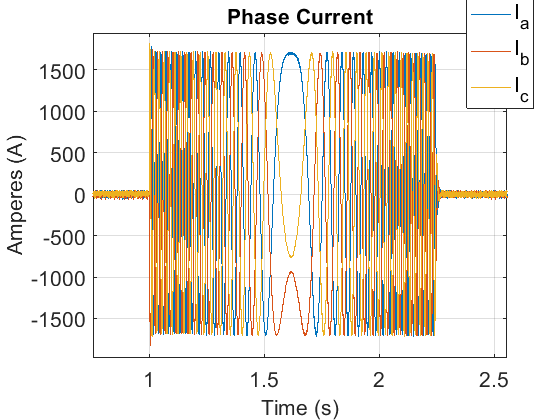
\includegraphics[width = 8 cm]{figs/reverse_sv_phase2.png}
            \caption{Line currents during reversal}
            \label{fig:r1}
        \end{subfigure}
        \hfill
        \begin{subfigure}[b]{0.475\textwidth}  
            \centering 
            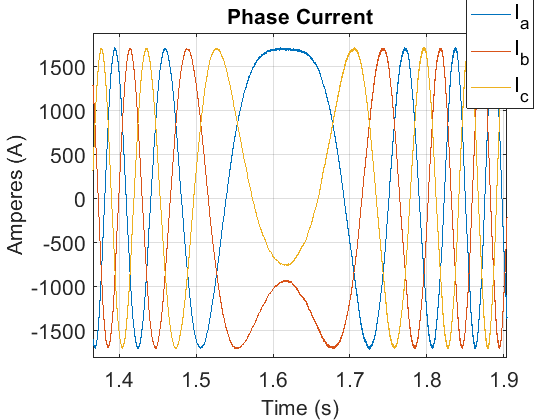
\includegraphics[width = 8 cm]{figs/reverse_sv_phase1.png}
            \caption{Line currents during rotation direction change}
            \label{fig:r2}
        \end{subfigure}
        \caption{Reversal, line currents}
        \label{fig:rev_line}
        \end{figure}

In the Fig. \ref{fig:dc2} below, we can see that our brake resistor starts operating voltage above 560, that is why in steady state we are constrained by 560V. Then, during the reversal due to the current supplied from the motor side, the voltage increases up to 580V, however, braking resistor allows us to discharge this energy. Then, the voltage is decreased to its final value after a transient period. When we have a look at Fig. \ref{fig:sc2} we can observe that in steady state both currents are zero with noise, however in the transient time, we have a negative $i_q$ resulted from the motor's reversal. This current discharges over the braking resistance.
        
\begin{figure}[H]
        \centering
        \begin{subfigure}[b]{0.475\textwidth}
            \centering
            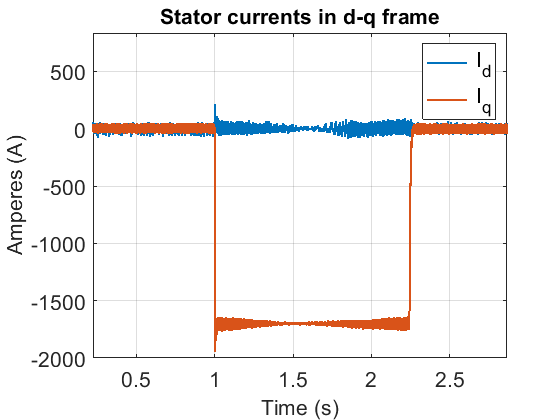
\includegraphics[width = 8 cm]{figs/reverse_sv_dq.png}
            \caption{Stator currents}
            \label{fig:sc2}
        \end{subfigure}
        \hfill
        \begin{subfigure}[b]{0.475\textwidth}  
            \centering 
            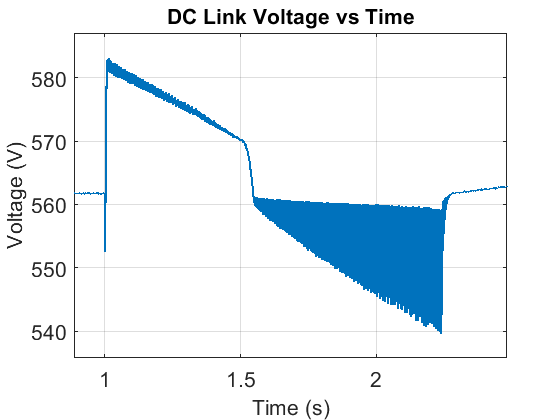
\includegraphics[width = 8 cm]{figs/reverse_sv_dc.png}
            \caption{DC link voltage}
            \label{fig:dc2}
        \end{subfigure}
        \caption{Reversal, d-q currents (a) and DC Link voltage (b)}
        \label{fig:dcc}
        \end{figure}        

\subsubsection{Q1-4}

Now, we need to speed up the motor to the 150\% rated speed. We need to control the current and voltage limits by doing so. First we need to fulfill the equation

\begin{equation}
    i_{s,max} \geq i_d^2 + i_q^2 
\end{equation}

and also:
\begin{equation}
 V_{max} = \sqrt{(\omega_e \lambda + i_d \omega_e L_d)^2 + (i_q \omega_e L_q)^2)}
\end{equation}

As we calculated from the previous part, the current $i_q$ necessary for both operations is:

\begin{equation}
     i_q = \dfrac{T_{m}}{3 \lambda }
\end{equation}

where Torque can be found as:
$$ T = 1273 Nm$$

When we calculate it:

$$ i_q = \dfrac{1273}{1.5} = 848.7A$$

In this case our $V_{max} = \dfrac{540}{\sqrt{3}} = 311V$ and we can calculate our minimum $i_d$ using this equation. As we can see below:

$$ 311 = \sqrt{235.5 - 0.165i_d)^2 + (140)^2) } $$

required $i_d = 0$. That means, we do not need to supply and $i_d$ current to operate in this speed with half of the torque. Now, let us show this in simulation!

\begin{figure}[H]
        \centering
        \begin{subfigure}[b]{0.475\textwidth}
            \centering
            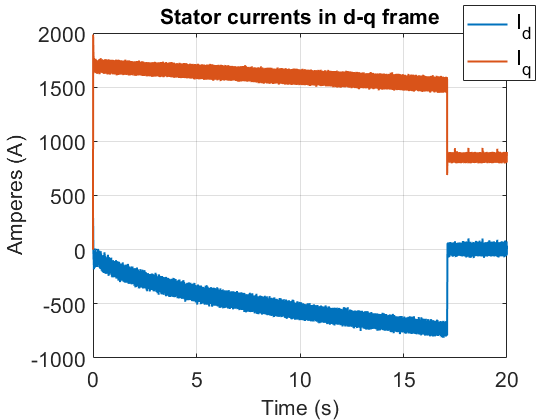
\includegraphics[width = 8 cm]{figs/c4_new_dq.png}
            \caption{Stator currents}
            \label{fig:c4_new_dq}
        \end{subfigure}
        \hfill
        \begin{subfigure}[b]{0.475\textwidth}  
            \centering 
            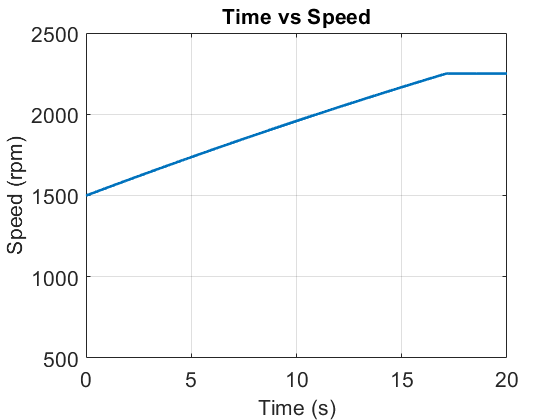
\includegraphics[width = 8 cm]{figs/c4_new_speed.png}
            \caption{Speed vs time}
            \label{fig:c4_new_speed}
        \end{subfigure}
        \caption{Field weakening, d-q currents (a) and speed vs time}
        \label{fig:c4}
        \end{figure}  


In the transient time, we need to apply the maximum $i_q$ current to obtain a fast transient. We need as much as torque we can supply to the system. However, at the steady state when the motor reaches its final value, we do not have to supply same amount of  $i_q$ or $i_d$. As we can see from the Fig.\ref{fig:c4} above, it is possible to operate with zero $i_d$ at that speed. It is possible because we are not operating in the maximum torque, and due to the SVPWM we have a larger margin for the field weakening!

\subsection{Q2}

In the Fig. \ref{fig:vref} below we can observe reference voltages for SVPWM and SPWM at rated operation conditions.

\begin{figure}[H]
        \centering
        \begin{subfigure}[b]{0.475\textwidth}
            \centering
            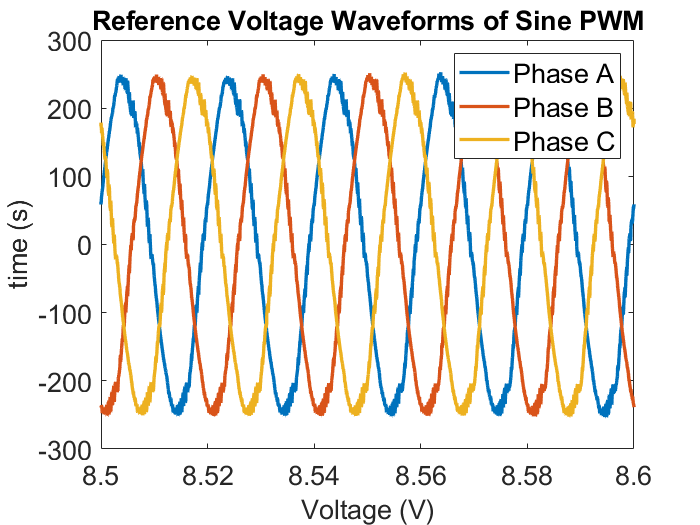
\includegraphics[width = 8 cm]{figs/sine_ref.png}
            \caption{SPWM}
            \label{fig:ref1}
        \end{subfigure}
        \hfill
        \begin{subfigure}[b]{0.475\textwidth}  
            \centering 
            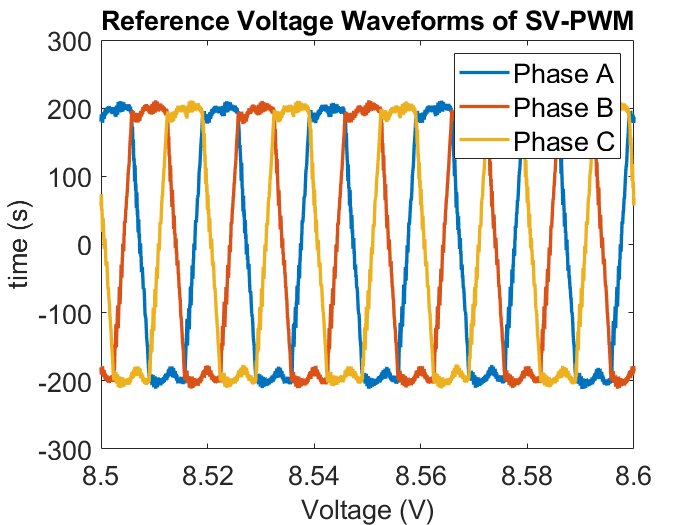
\includegraphics[width = 8 cm]{figs/svpwm_ref.png}
            \caption{SVPWM}
            \label{fig:ref2}
        \end{subfigure}
        \caption{Voltage reference waveforms in three phase, SPWM (a) and SVPWM (b)}
        \label{fig:vref}
        \end{figure}  


%% comments here !!!

Reference voltages of SVPWM are different from reference voltages of SPWM. In SVPWM, duration times of $V_7$ and $V_0$ space vectors  are equal, it means that both zero vectors are equal time applied to the circuitry, but in SPWM these durations are not equal and they are determined by analog comparators. This is the reason why two reference voltages are different. Moreover, we should notice that the total phase voltage of the SVPWM is much higher than the SPWM $V_{spwm} = \frac{V}{2} $ and $V_{svpwm} = \frac{V}{\sqrt{3}} $. This is due to the reference voltages and their durations. The above-mentioned phenomenon that zero vector durations are the same for SVPWM results in a higher phase voltage. That is why in high voltage applications SVPWM is the chosen one.

Above in the Fig. \ref{fig:vref} we should also notice that both methods generate same current, however SVPWM has less peak in the voltage reference, which means it is possible to have larger voltages with SVPWM, where it is not possible for SPWM.


\subsection{Q3}

In the Fig. \ref{fig:thd} below we can observe the THD analysis of SVPWM and SPWM methods.

\begin{figure}[H]
        \centering
        \begin{subfigure}[b]{0.475\textwidth}
            \centering
            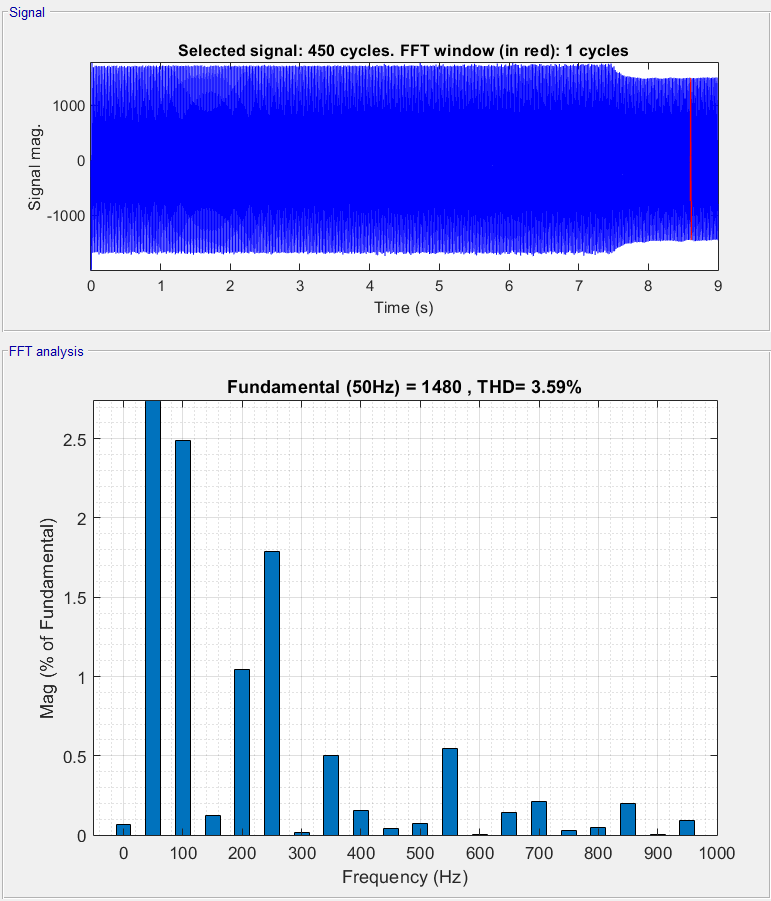
\includegraphics[width = 7 cm, height = 9 cm]{figs/FFT_Sine_PWM.PNG}
            \caption{SPWM}
            \label{fig:thd_s}
        \end{subfigure}
        \hfill
        \begin{subfigure}[b]{0.475\textwidth}  
            \centering 
            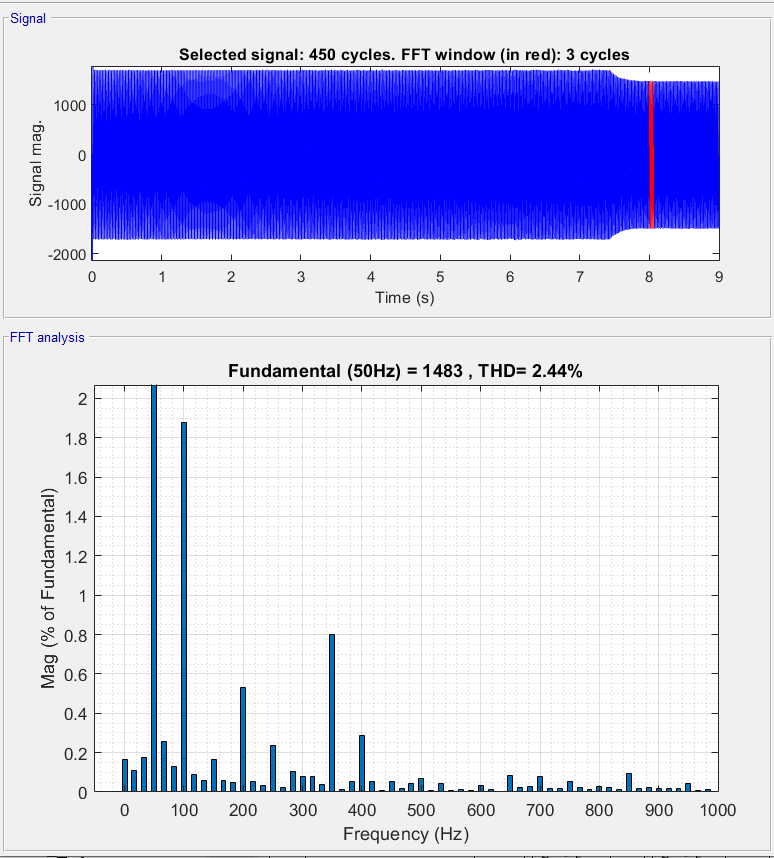
\includegraphics[width = 7 cm, height = 9 cm]{figs/FFT_SVPWM.PNG}
            \caption{SVPWM}
            \label{fig:thd_sv}
        \end{subfigure}
        \caption{THD Analysis of both methods SPWM (a) and SVPWM (b)}
        \label{fig:thd}
        \end{figure}  
        

\begin{center}
\begin{figure}[H]
\centering
\includegraphics [width= 12 cm]{figs/THD_sv.png}
\caption{THD Analysis in switching frequencies}
\label{fig:thd_switch}
\end{figure}
\end{center}
        
        

%COMMENTS HERE 

Above, we can see that SVPWM has 2.44\% THD, and SPWM has 3.6\% THD. From FFT analysis we can see that in both methods, there is no third harmonics due to the three phase inverter. Actually, we did not expect any harmonics around fundamental frequencies but due to the simulation and non-ideality of our PWM generation techniques, we have some harmonics around the fundamental frequency. Most importantly the THD values of both applications is very low. Also, this THD analysis is done in the rated current, which means it is done in the $m_a = 1$. If we are to decrease this value, then the THD of both line currents would be higher. Moreover, magnitudes of the harmonics are less in SVPWM comparing to the SPWM. Therefore, THD of SVPWM is less than SPWM. This means that SVPWM uses DC voltage with less harmonics, which means the power factor of SVPWM line current will be higher comparing to the SVPWM.

Also, it is essential to see that THD of SVPWM varies less comparing to the SPWM, in smaller ratios of $m_a$ SPWM would show more harmonics, where SVPWM would show less.

When we look at the Fig. \ref{fig:thd_switch} we can see that around the $f_s$ and its multiples we can see harmonics. These harmonics are determined by the modulation ratio, and unipolar switching characteristics. We can see that since we are applying a unipolar switching strategy, the harmonics are very very low, and it effects total harmonics a very little value!




\subsection{Q4}

For high performance drive, SVPWM is better choice. 
\begin{itemize}
    \item Firstly, it has less switching losses because when the voltage changes, only one switch changes its states. In SPWM this is not the case, and multiple switchings cause higher losses on the switches.
    \item Another advantage of SVPWM is that is uses less DC voltage to reach same line-to-line voltage, this is due to harmonics of the both application methods. SVPWM is better in harmonics.
    \item In high voltage applications, SVPWM is more advantageous due to its high voltage capability. It caries almost 15\% more voltage than the SPWM in applications and when we think of applications in kV range, this means a lot.
\end{itemize}

The reasons itemized above shows that SVPWM is a better choice for high performance applications, its digital nature and hand made zero vector selections makes it a better choice against the SPWM method. However, the necessity of a digital controller and the effort to implement it is higher than the SPWM. In this project, it was very hard to implement SVPWM where SPWM was very easy to implement at all.

\end{document}